% PART II — MATHEMATICAL & ALGORITHMIC FOUNDATIONS
\chapter{Chapter 3: Reinforcement Learning, SAC, HER, Imitation, Randomization, and HRL}
\section{3.1 Goal-Conditioned Markov Decision Processes and Soft Actor-Critic (SAC)}
A. Definition \& Role: Task execution is modeled as a Goal-Conditioned MDP (S, A, G, P, r, gamma), where observations follow the Gymnasium GoalEnv Dict schema {observation, achieved\_goal, desired\_goal}. Soft Actor-Critic (SAC) is an off-policy maximum-entropy actor-critic algorithm that simultaneously maximizes expected discounted return and expected policy entropy H(pi(.|s,g)).

B. Internal Mechanics \& Equations: SAC trains twin Q-critics Q\_{theta\_1}, Q\_{theta\_2} against Polyak-averaged targets (tau=0.05 early; 0.005 late) using clipped double-Q minimization to curb overestimation bias (Equations 3–4). The stochastic actor samples continuous 4D actions via the reparameterization trick a = tanh(mu\_phi(s,g) + sigma\_phi(s,g)*eps) and optimizes Equation (5), while automatic Lagrange dual updates adapt temperature alpha toward target entropy H\_tgt = -dim(A) = -4 (Equation 6).

\begin{figure}[htbp]\centering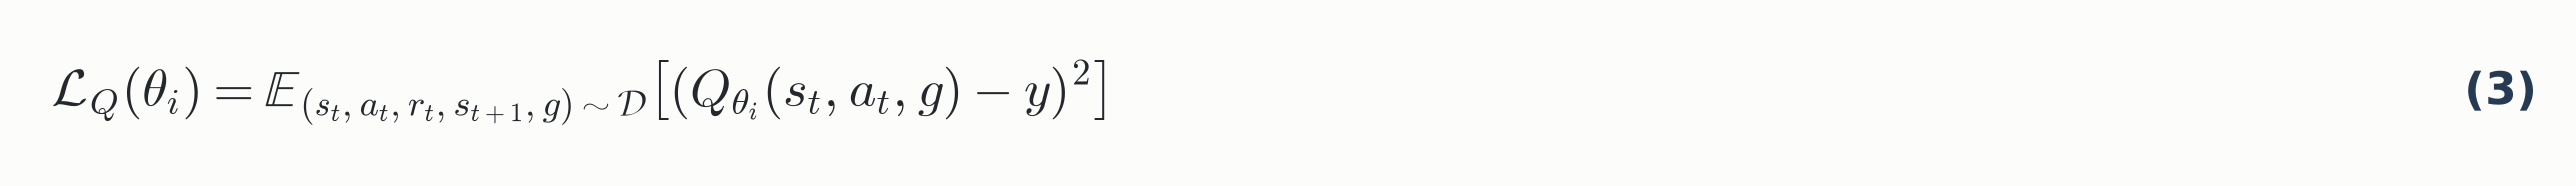
\includegraphics[width=0.9\linewidth]{../../assets/equations/eq_03.png}\caption{Equation (3): Clipped double Q-learning critic regression objective.}\end{figure}
\begin{figure}[htbp]\centering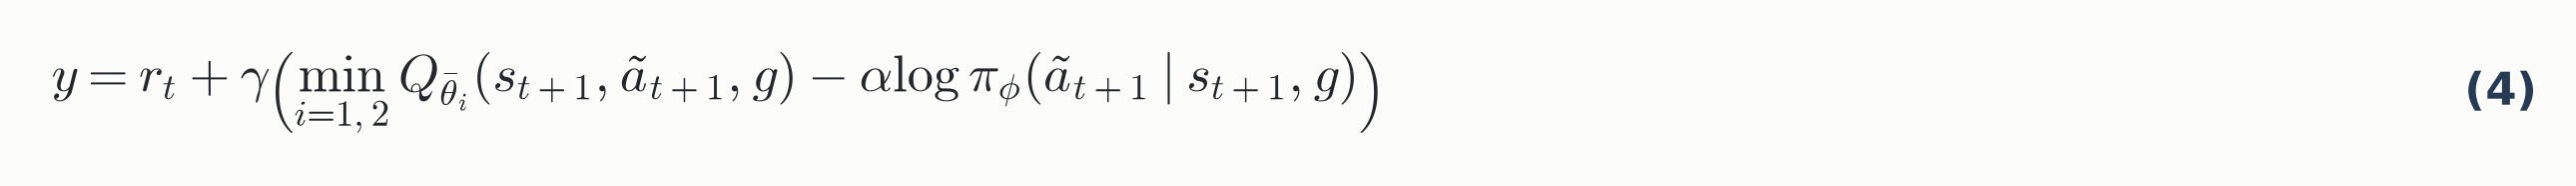
\includegraphics[width=0.9\linewidth]{../../assets/equations/eq_04.png}\caption{Equation (4): Soft Bellman backup target with entropy bonus.}\end{figure}
\begin{figure}[htbp]\centering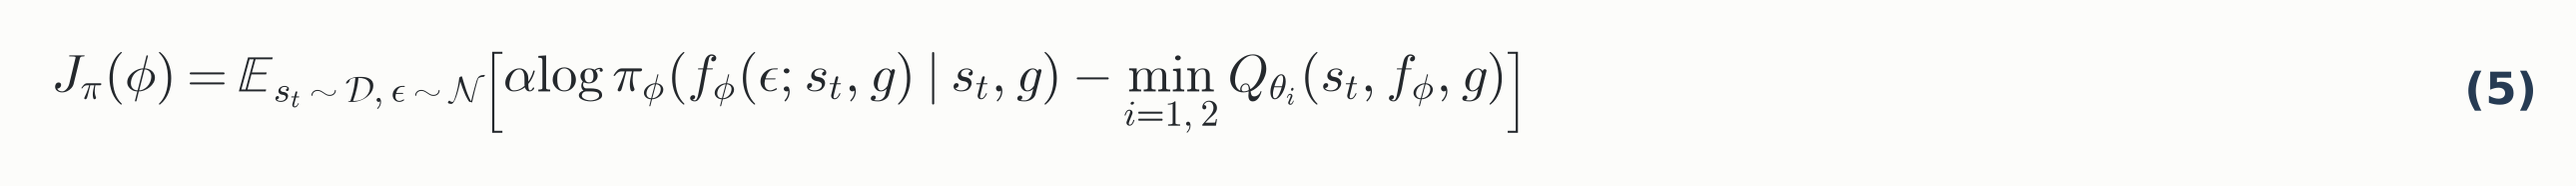
\includegraphics[width=0.9\linewidth]{../../assets/equations/eq_05.png}\caption{Equation (5): Reparameterized SAC actor objective.}\end{figure}
\begin{figure}[htbp]\centering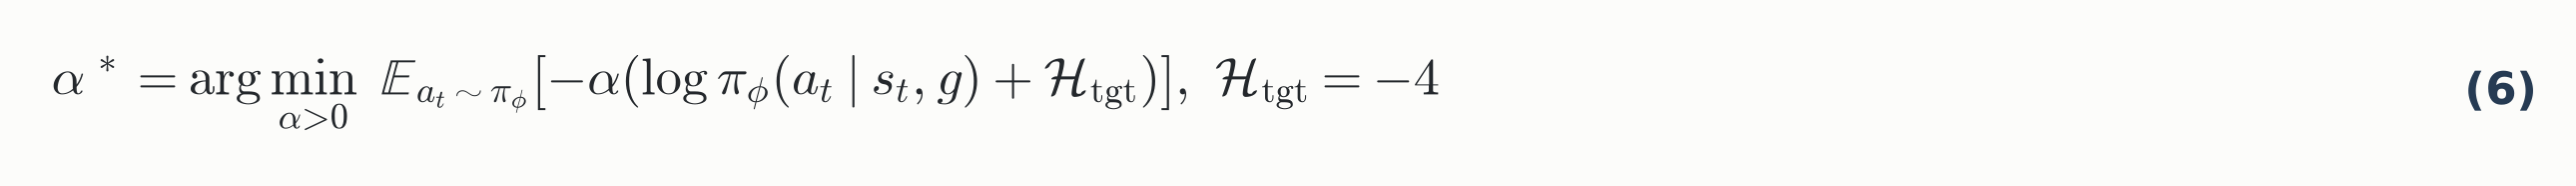
\includegraphics[width=0.9\linewidth]{../../assets/equations/eq_06.png}\caption{Equation (6): Automatic entropy temperature dual minimization.}\end{figure}
C. Alternatives, Limitations \& Evidence: On-policy methods like PPO discard off-policy replay transitions and lack native HER compatibility; deterministic off-policy methods like DDPG/TD3 require external exploration noise tuning. Across 10k sparse runs in Phases 2–8, SAC suffered premature alpha collapse (0.907 -> 0.002), demonstrating that without informative positive gradients, entropy scheduling alone cannot bridge long manipulation horizons.

\section{3.2 Hindsight Experience Replay (HER) and Sparse vs. Dense Reward Shaping}
A. Mechanism \& Static-Goal Exploration Trap (ERR-003): Under binary sparse rewards r = -I(||p\_obj - p\_goal|| > 0.05 m) (Equation 7), random policies almost never hit desired goals. Future-strategy HER (k=4, Equation 8) retrospectively substitutes achieved states g' = ag\_tau (tau > t) into replay mini-batches, turning failed trajectories into valid goal-reaching examples. However, Phase 11 (25 models x 100k steps = 0.0\% across 5,000 evaluation episodes) uncovered a critical failure mode: when an agent fails even to move the object off the table, every future achieved goal g' equals the static initial resting coordinate, reinforcing stationary hovering.

\begin{figure}[htbp]\centering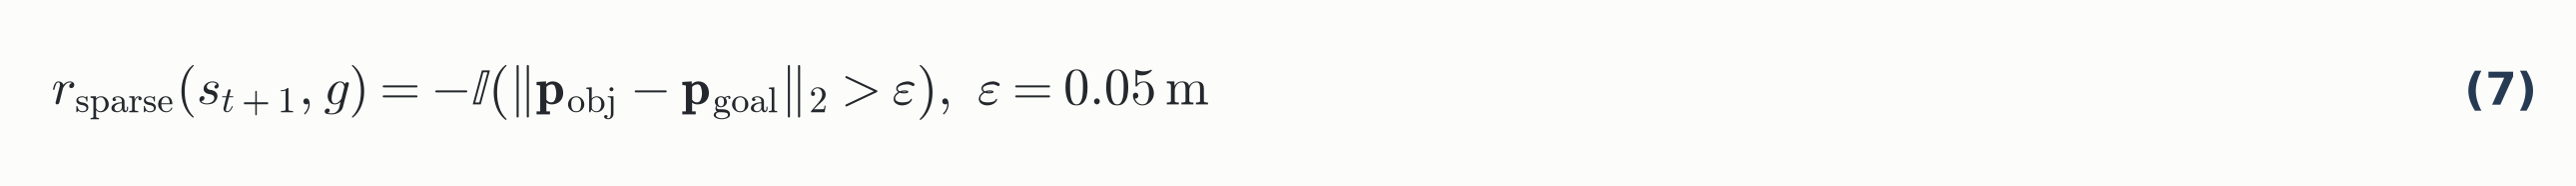
\includegraphics[width=0.9\linewidth]{../../assets/equations/eq_07.png}\caption{Equation (7): Binary sparse Euclidean tolerance reward.}\end{figure}
\begin{figure}[htbp]\centering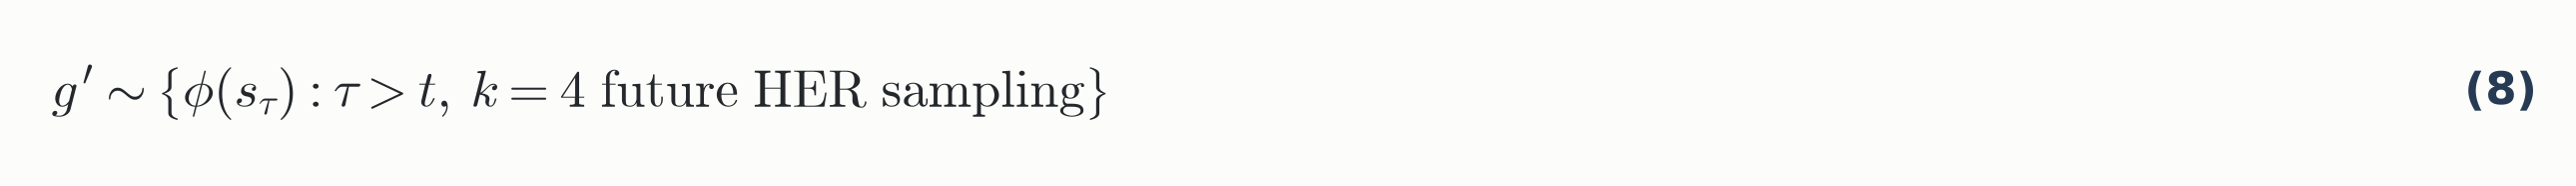
\includegraphics[width=0.9\linewidth]{../../assets/equations/eq_08.png}\caption{Equation (8): Future-strategy HER virtual goal relabeling (k=4).}\end{figure}
\begin{figure}[htbp]\centering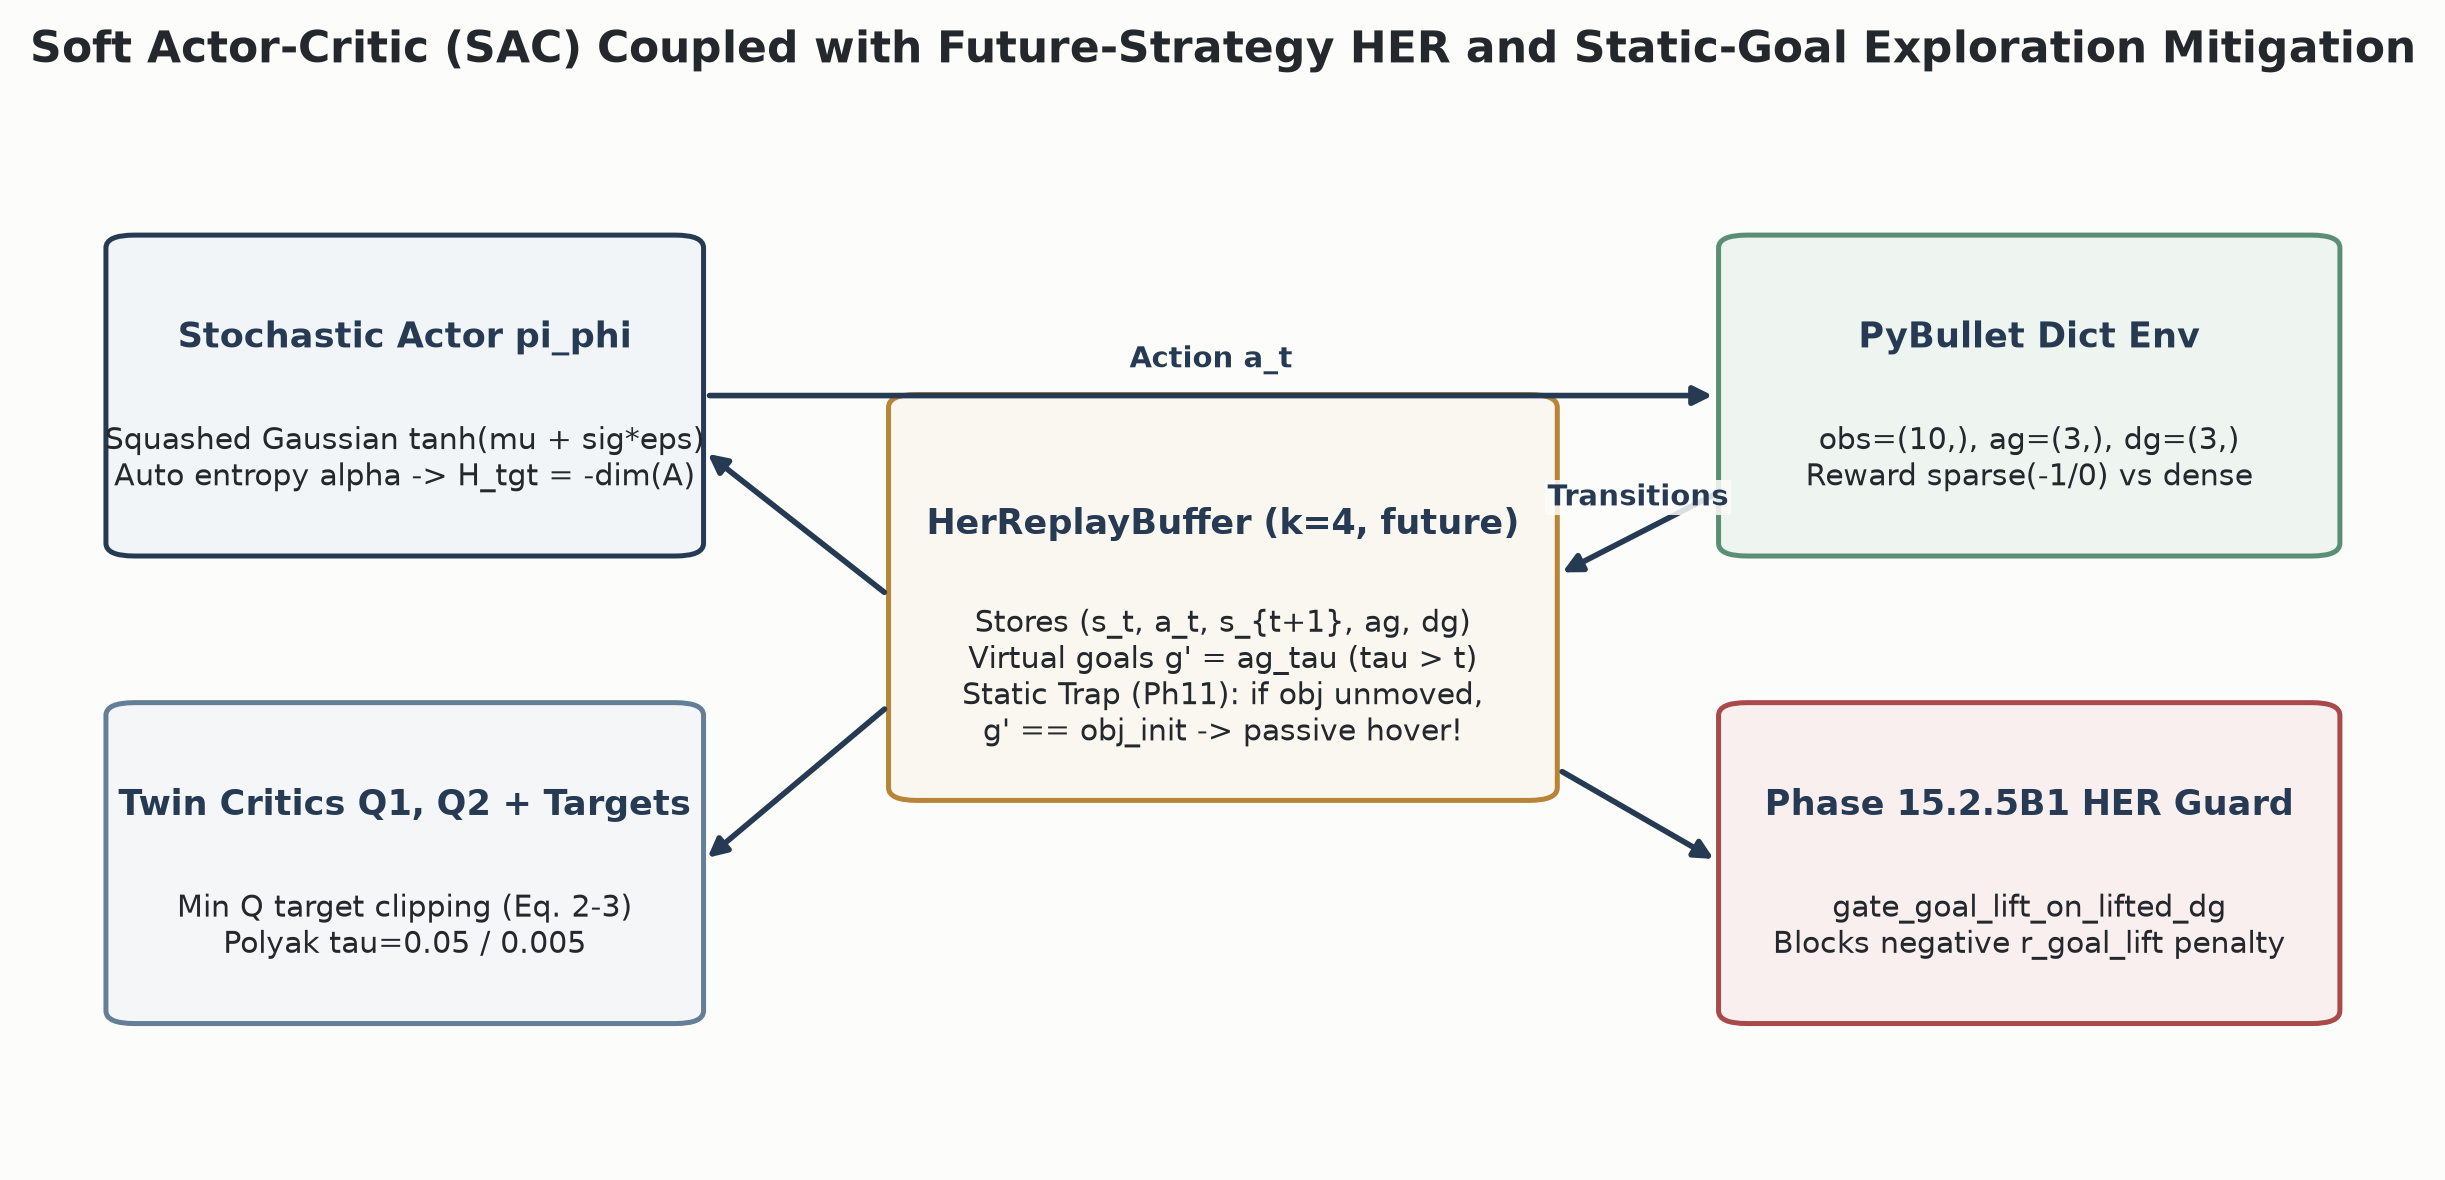
\includegraphics[width=0.9\linewidth]{../../assets/diagrams/diag_06_sac_and_her_architecture.png}\caption{Figure 3.1: Off-policy SAC actor-critic dataflow coupled with HER k=4 virtual relabeling and the Phase 15.2.5B1 lift-gradient guard.}\end{figure}
B. Dense Staged Shaping \& Continuous Vertical Potentials: Breaking the static trap in Phase 12 required staged dense shaping (Equation 10) uniting approach attraction, bilateral contact bonuses, lift altitude increments, goal transport potential, and collision penalties. Similarly, Phase 15.2.5B1 overcame an XY-gated vertical hover deadlock at z=0.50 m by replacing cylinder-gated Z rewards with an un-gated continuous vertical potential Phi\_z = -2.0 * clip(|z\_ee - z\_grasp|, 0, 1) (Equation 11).

\begin{figure}[htbp]\centering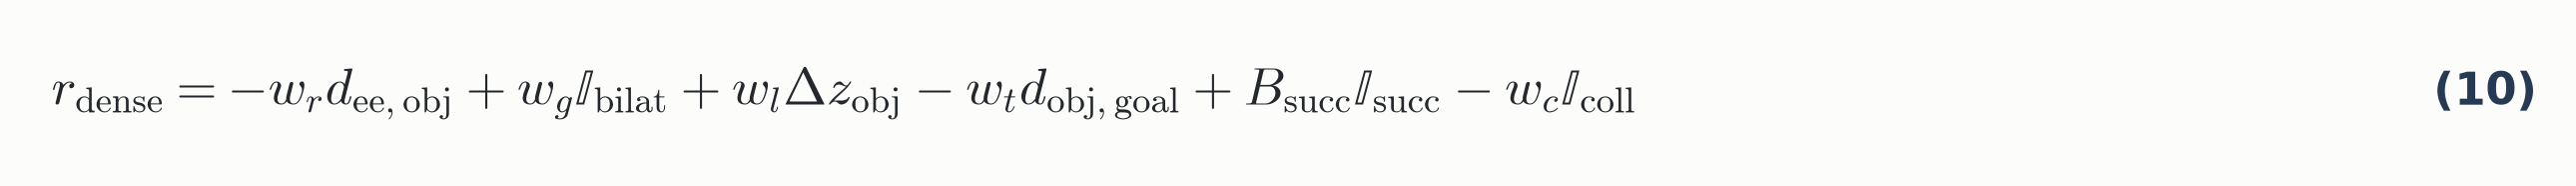
\includegraphics[width=0.9\linewidth]{../../assets/equations/eq_10.png}\caption{Equation (10): Multi-stage dense manipulation shaping function (Phase 12).}\end{figure}
\begin{figure}[htbp]\centering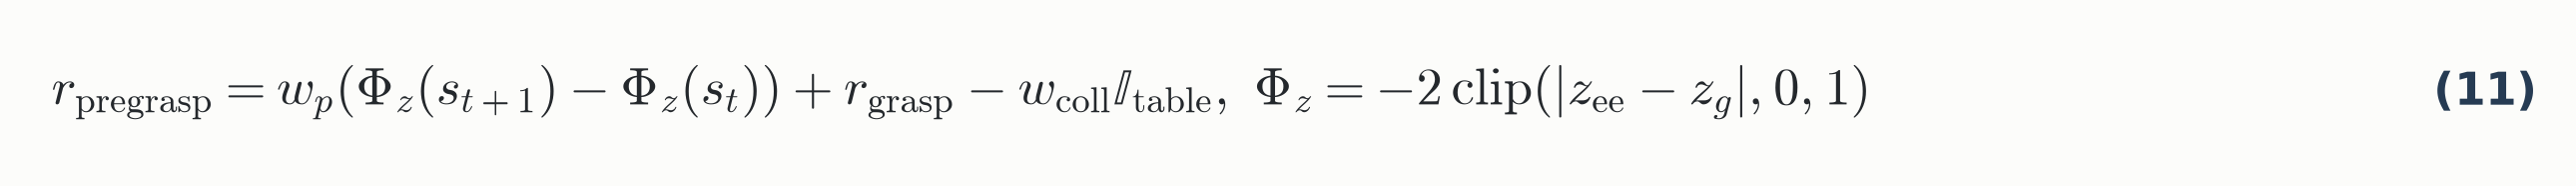
\includegraphics[width=0.9\linewidth]{../../assets/equations/eq_11.png}\caption{Equation (11): Continuous un-gated vertical approach potential Phi\_z (Phase 15.2.5B1).}\end{figure}
\begin{figure}[htbp]\centering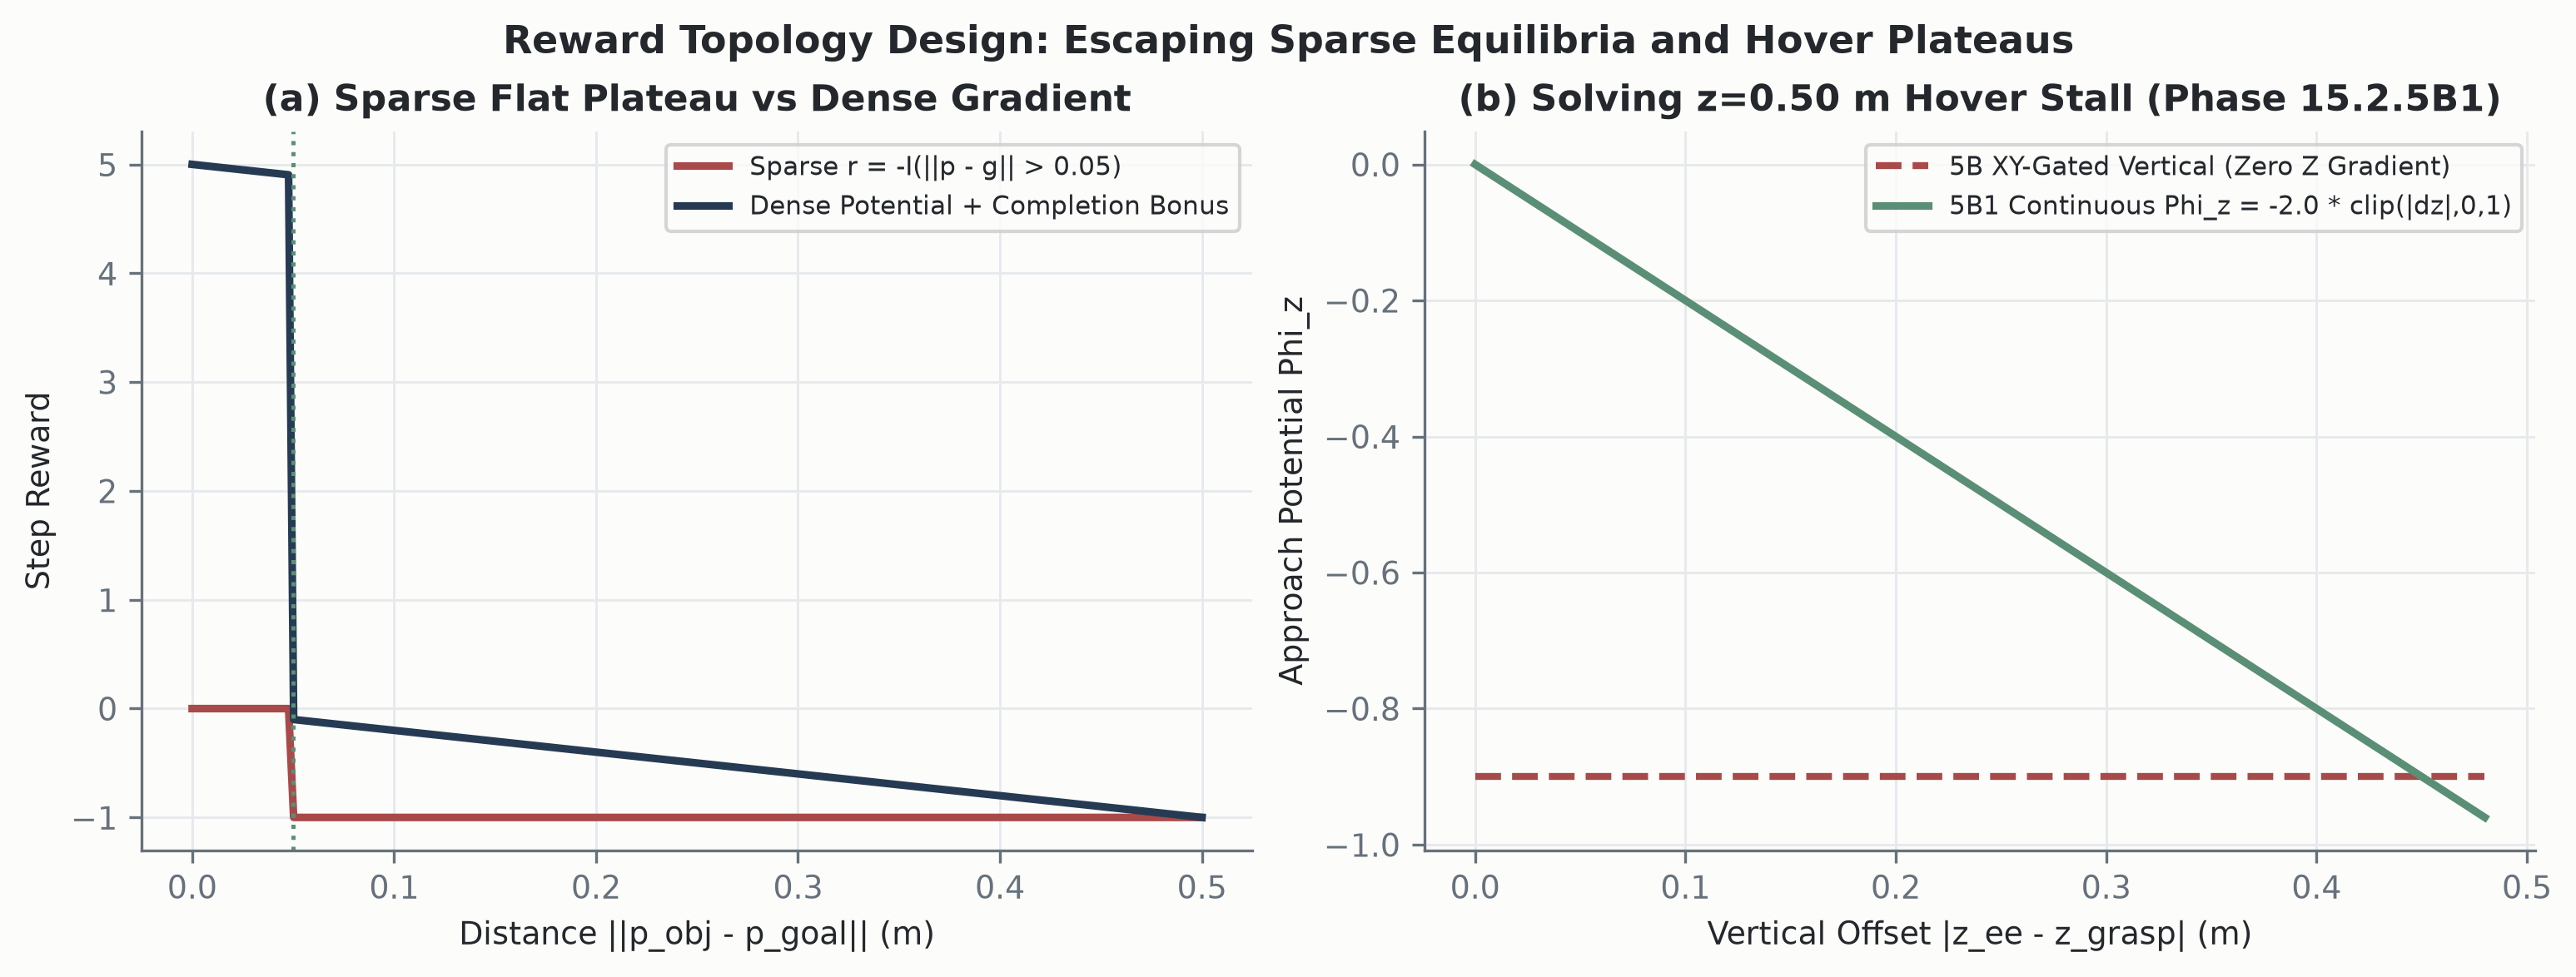
\includegraphics[width=0.9\linewidth]{../../assets/diagrams/diag_14_reward_shaping_potential.png}\caption{Figure 3.2: (a) Sparse plateau vs. dense gradient; (b) Solving the z=0.50 m hover stall via un-gated vertical potential Phi\_z.}\end{figure}
\section{3.3 Progress-Masked Behavioral Cloning, Hybrid BC-SAC, Domain Randomization \& HRL}
Behavioral Cloning (BC) initializes actor policies from expert demonstrations via supervised regression. Phase 15.2.5B.1 proved that naive BC over complete scripted episodes overfits trailing stationary HOLD\_AT\_GOAL frames (78.4\% closed-jaw bias), causing premature air-pinching. Introducing balanced open-approach demos (70.1\% open descent) and binary progress masking M\_prog(s) (Equations 12–13) propelled pure masked BC (5B7) to 75\% grasp and 45\% lift across 100 episodes with 0\% table collisions, while Decaying Hybrid BC-SAC (5B8) reached 66\% / 26\%.

\begin{figure}[htbp]\centering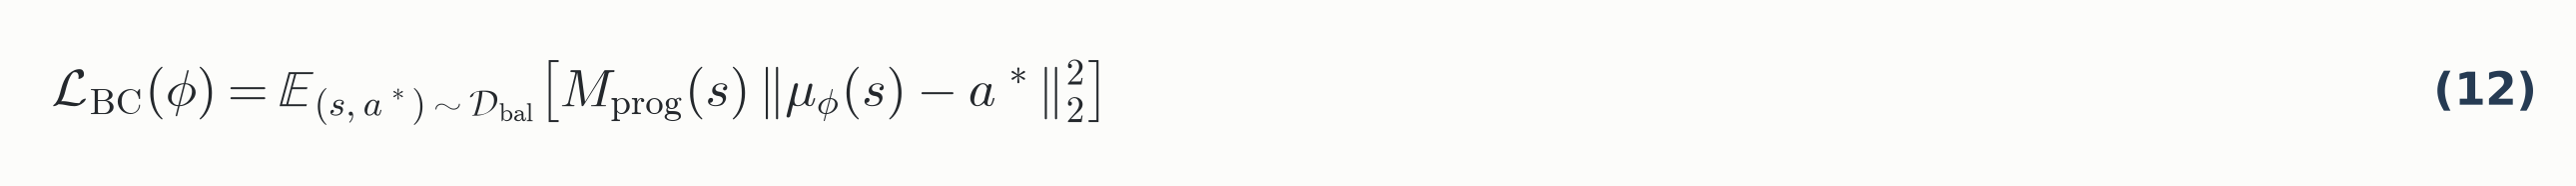
\includegraphics[width=0.9\linewidth]{../../assets/equations/eq_12.png}\caption{Equation (12): Progress-masked Behavioral Cloning L2 objective.}\end{figure}
\begin{figure}[htbp]\centering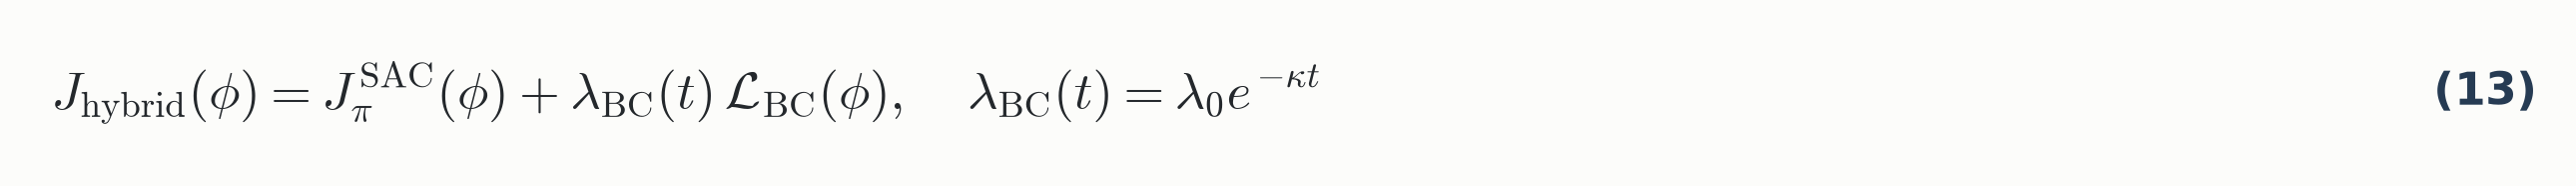
\includegraphics[width=0.9\linewidth]{../../assets/equations/eq_13.png}\caption{Equation (13): Exponentially decaying Hybrid BC-SAC objective with entropy floor.}\end{figure}
\begin{figure}[htbp]\centering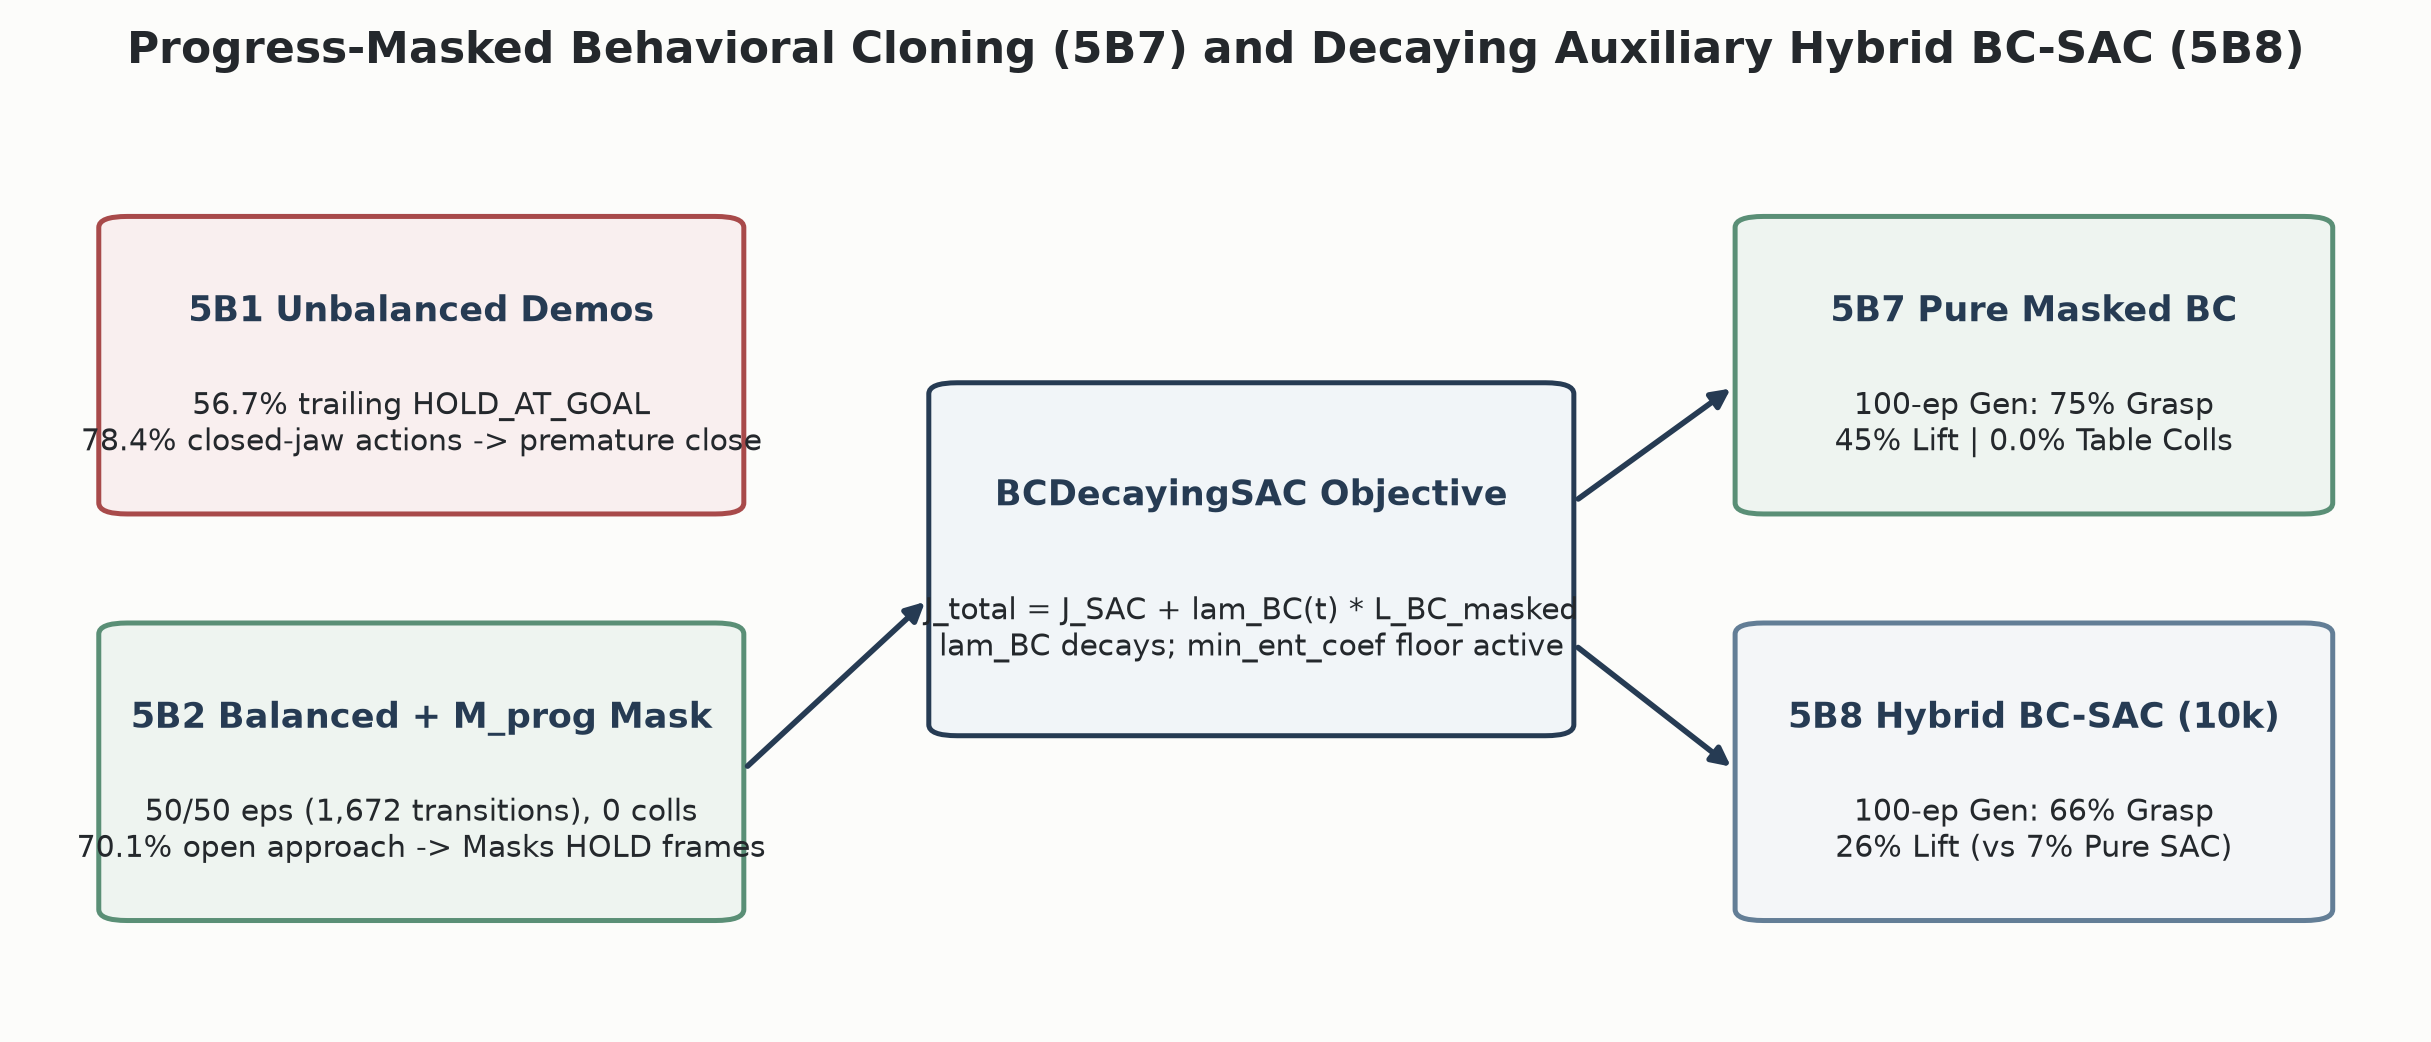
\includegraphics[width=0.9\linewidth]{../../assets/diagrams/diag_07_bc_and_hybrid_bcsac.png}\caption{Figure 3.3: Transition from unbalanced closed-jaw BC bias (5B1) to balanced masked BC (5B7) and decaying Hybrid BC-SAC (5B8).}\end{figure}
Domain Randomization (DR0–DR4, Figure 3.4) varies cube mass (0.04–0.25 kg), Coulomb friction (0.3–1.5), and spawn/goal geometry so policies do not overfit fixed nominal constants. Hierarchical RL (Phase 16.1, Equation 14) further mitigates horizon complexity by training a high-level discrete meta-policy pi\_high(u|s) over five modular closed-loop skill policies {REACH, ALIGN, GRASP, LIFT, TRANSPORT}.

\begin{figure}[htbp]\centering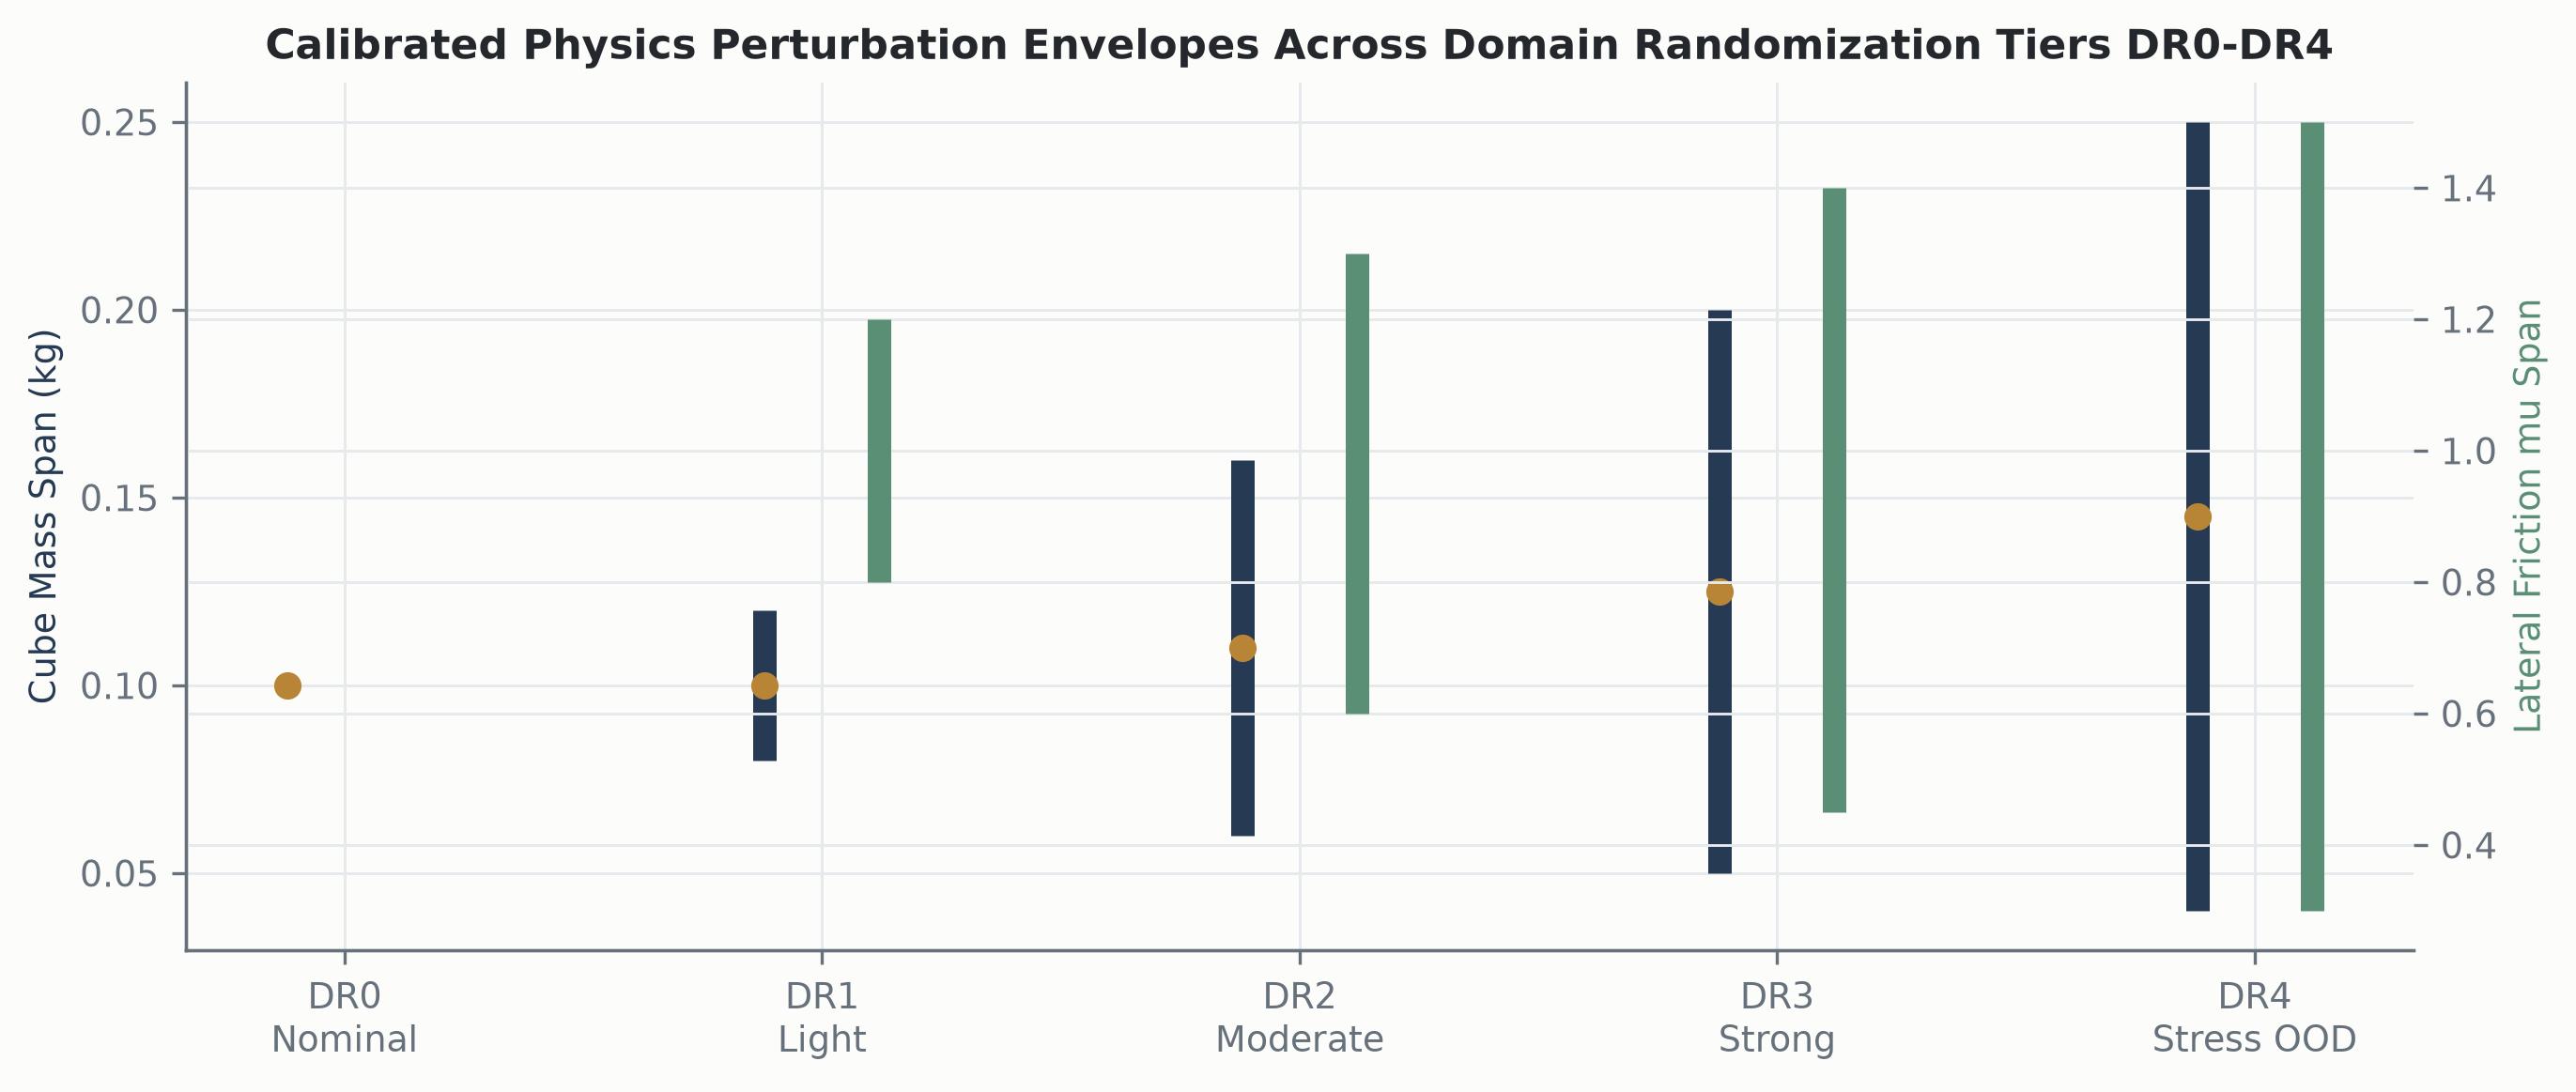
\includegraphics[width=0.9\linewidth]{../../assets/diagrams/diag_08_domain_randomization_dr0_4.png}\caption{Figure 3.4: Calibrated physical mass and friction parameter spans across Domain Randomization tiers DR0 through DR4.}\end{figure}
\begin{figure}[htbp]\centering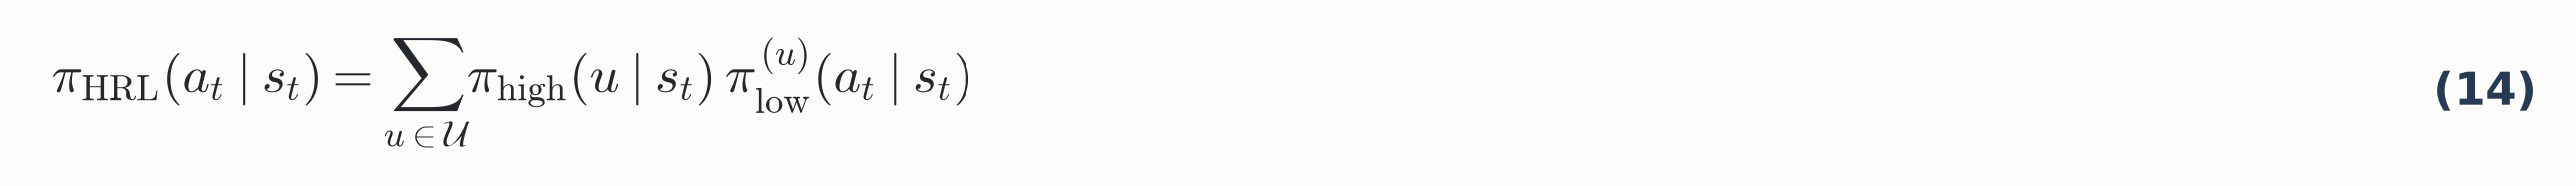
\includegraphics[width=0.9\linewidth]{../../assets/equations/eq_14.png}\caption{Equation (14): Five-skill hierarchical option policy marginalization (Phase 16.1).}\end{figure}